\chapter{Implementation}


At the beginning of the implementation I used the data model for abstract part that can be produced on any machine. Using Hyperledger Composer Modelling Language I defined assets, queries and participants. 
Since the model is very straightforward it was easy to describe it. Code is self explanatory.

\begin{figure}[H]
    \begin{center}
        \begin{minipage}{\linewidth}
            \begin{center}
                \shadowimage[width=(\textwidth),keepaspectratio]{img/code_assets.png}
                \caption{Asset code}
                \label{obr 1.2.1}
            \end{center}
        \end{minipage}
    \end{center}
\end{figure}

Chain code is installed on every peer and is responsible for executing transactions. Our transaction logic is simple and only thing that peers have to agree on is change of the product owner. Input variable \inlinecode{trade} contains new owner and product. Very important aspect of the chaincode is \inlinecode{@transaction} and \inlinecode{param} pragmas which are used to distinguish transaction code. This code is also emitting an event about the transaction so we can subscribe to the events in future.  

\begin{figure}[H]
    \begin{center}
        \begin{minipage}{\linewidth}
            \begin{center}
                \shadowimage[width=(\textwidth),keepaspectratio]{img/code_trade.png}
                \caption{Transaction code}
                \label{obr 1.2.1}
            \end{center}
        \end{minipage}
    \end{center}
\end{figure}


Thanks to Composer I was able to quickly model and deploy configuration of the network which took considerable amount of time compared to pure Fabric. To deploy blockchain network we have to firtly define high level definition of our topology. Fabric standards use \inlinecode{crypto-config.yaml} file to define system. Creating single user in this definition means to create one more user that is not an admin. Increasing number of peers would lead to generation of more peers but also higher performance demands which I wanted to avoid, especially when using virtual machine and not so powerful hardware.


\begin{figure}[H]
    \begin{center}
        \begin{minipage}{\linewidth}
            \begin{center}
                \shadowimage[width=(\textwidth),keepaspectratio]{img/code_crypto_config.png}
                \caption{Crypto-config definition}
                \label{obr 1.2.1}
            \end{center}
        \end{minipage}
    \end{center}
\end{figure}

This YAML file is then provided as an input paramater to Fabric's  \inlinecode{cryptogen} tool for generating Hyperledger Fabric key material. Cryptogen will generate all the certificates for peers and other network components

\begin{figure}[H]
    \begin{center}
        \begin{minipage}{\linewidth}
            \begin{center}
                \shadowimage[width=(0.5\textwidth),keepaspectratio]{img/crypt-gen-folder.png}
                \caption{Structure of crypto-gen}
                \label{obr 1.2.1}
            \end{center}
        \end{minipage}
    \end{center}
\end{figure}

All of the network components are secured using Transport Layer Security to encrypt communications. Certificate Authority has to create certificates for all of the network components in order to connect to those network components. The CA certificates can be found in the directory \inlinecode{crypto-config} with suffix \inlinecode{ca.crt}.

YAML file above describes topology of the network. Connection profiles with necessary certificates and addresses for connection to network components are described in \inlinecode{byfn-network.json}. This file is very important because it contains every certificate that I have generated using CA to encrypt communication over network. To avoid mistakes I copied corresponding certificates and private keys to a temporary folder for every organization and carefully defined certificates for specific peers and CA. 

\section{Deployment}

Business network card is created using \inlinecode{composer card create} command with specified connection profile for the organisation and certificates. Network card is an archive which contains connection details and certificates. Since we have two organisations \emph{org1} and \emph{org2} I created two different cards for the administrator to use to deploy the blockchain business network to the Hyperledger Fabric network.
These cards are further used to install the business network onto Fabric. 
Using this command I install business network on peers within \emph{org1}. Analogically on \emph{org2}
\begin{lstlisting}
composer network install --card PeerAdmin@byfn-network-org1 --archiveFile vortex-network.bna
\end{lstlisting}

After deployment of administrator on network we can proceed and create cards for customer access. I created cards  \emph{customera} for \emph{org1} and \emph{customerb} for \emph{org2}. 
\begin{lstlisting}
composer card create -p ./tmp/composer/org1/byfn-network-org1.json -u customera -n vortex-network -c customera/admin-pub.pem -k customera/admin-priv.pem
composer card import -f customera@vortex-network.card
\end{lstlisting}

Now we can use this business network card to interact with the blockchain business network and onboard other participants in your organization. Every operation on the network has to identified. To invoke chaincode or interact with the network the network card has to be specified as a paramater of every command. 

To avoid writing long commands I used Composer REST server to interact with the network. Hyperledger Composer includes a standalone Node.js process that exposes a business network as a REST API. The LoopBack framework is used to generate an Open API, described by a Swagger document. Following command will start a server listening at port 3000 for \emph{customerb} to interact with the network. 

\begin{lstlisting}
composer-rest-server -c customerb@vortex-network -n never -u true -w true
\end{lstlisting}

If everything works, after entering \inlinecode{localhost:3000} into our browser we should be able to see web interface generated for us.

\begin{figure}[H]
    \begin{center}
        \begin{minipage}{\linewidth}
            \begin{center}
                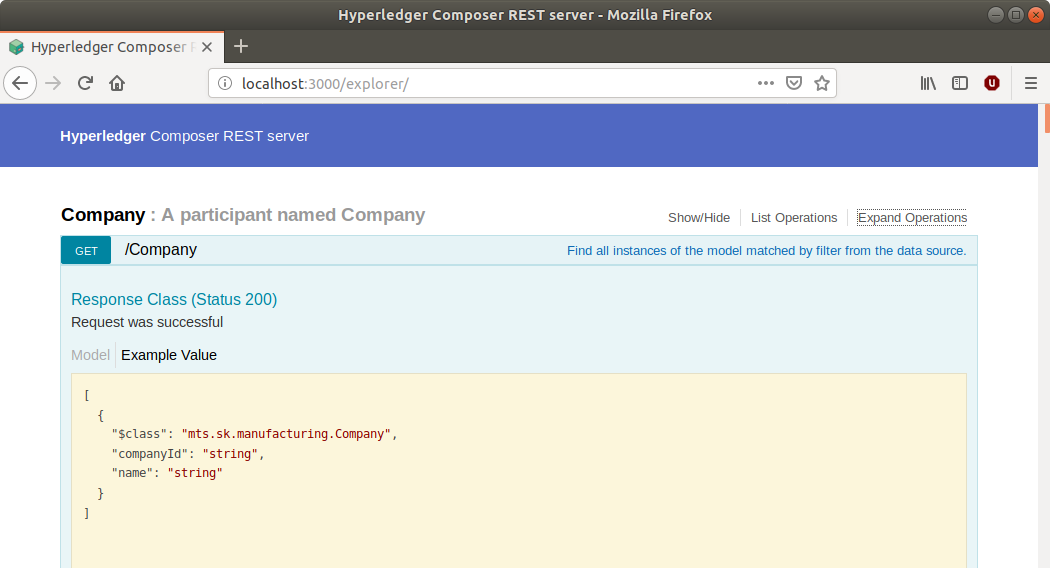
\includegraphics[width=(\textwidth),keepaspectratio]{img/composer_server.png}
                \caption{Hyperledger Composer REST server}
                \label{obr 1.2.1}
            \end{center}
        \end{minipage}
    \end{center}
\end{figure}

Having a running REST API for our blockchain network now means that we can make simple HTTP requests to the server from any application using almost every programming language we want. Generated API consists of  \emph{GET}, \emph{POST}, \emph{PUT}, \emph{HEAD} operations for managing Products, Companies, Trades and network logs. These operations follow REST standarts. 
                
When accessing blockchain network through API due to the level of abstraction it provides, it may appear to the user as a regular database. To see concrete blocks of the blockchain I wrote a simple application that uses \emph{composer-client native API} to read data in blockchain. It's simple application written in NodeJS using Express.JS framework to quickly write and deploy REST server. This application is connecting through native API and \emph{vortex-channel} to the network. 

This application is listening on port \emph{3001} and URLs described bellow.

\begin{table}[H]
\centering
\caption{ExpressJS application endpoint}
\begin{tabular}{|l|l|}
\hline
\textbf{URL}       & \textbf{Description}                                                                                                                         \\ \hline
\emph{GET} \textbackslash{blocks}\textbackslash{:id}             & Block {id} data                                                                                              \\ \hline
\emph{GET}  \textbackslash{queryInfo}\textbackslash             & Data about block height, current and previous hash data   \\ \hline

\end{tabular}
\end{table}

When accessing the blocks through \emph{blocks} interaface we can see data about the current specified block as JSON response. 

\begin{lstlisting}
  "header": {
    "number": "13",
    "previous_hash": "f6c3076842836a3fbc5f5306f73ac214804586ed5df18b3acea55383c1afcfea",
    "data_hash": "f4b1a0b59aa4d2469beed703b90921b326a1a575ab730bd8de942f7914a04a35"
  },
  "data": {
    "data": [
      {
        "signature": {
          "type": "Buffer",
          "data": [
            48,
            68,
            ...
            ]
\end{lstlisting}

Block data stores data in byte arrays and displays certificates of all nodes that were involed. When we query previous block in the chain, the \emph{previous   hash} would not match the data hash. That's beacuse a block hash is calculated by hashing over the concatenated ASN.1 encoded bytes of: the block number, previous block hash, and current block data hash.

Queryinfo endpoint queries for various useful information on the state of the Channel like height and known peers.  

Since the network is deployed in virtual machine I needed a way to connect to the REST server from hosting operating system. To achieve this connection I used \emph{Nginx} and defined a proxy pass on the port 80.

\begin{lstlisting}
server {
	listen 80 default_server;
	listen [::]:80 default_server;
	server_name _;
	location / {
		proxy_pass http://127.0.0.1:3000;
	}
	location /blocks/ {
		proxy_pass http://127.0.0.1:3001/;
}
\end{lstlisting}

This configuration takes care of requests made to the computer using http port 80  and forwards them to the application running on specific port on the local computer. Virtual machine IP address has to be in the same sub-net as is the application making requests to the server.

\section{Integration with manufacturing software}

Company MTS is using Beckhoff's PLCs with TwinCAT and develops its own software solution called \emph{Vortex} which allows easy integration with PLC code and development of complex software solutions which can satisfy costumer needs. Proprietary human machine interface (HMI) is replaced with widely used WPF and allows to use .NET framework with C\#. Modular architecture of this solution allowed easy integration of new data persistence. 

When a new product is assembled, PLC will execute command which invokes remote procedure on the PC side. Vortex is able to read whole objects in PLC as C\# objects. Generated code contains extension functions for storing plain objects without all the meta data in database. 

\begin{figure}[H]
    \begin{center}
        \begin{minipage}{\linewidth}
            \begin{center}
                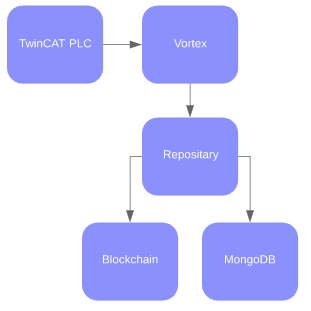
\includegraphics[width=(0.5\textwidth),keepaspectratio]{img/vortex_data.png}
                \caption{Storing data }
                \label{obr 1.2.1}
            \end{center}
        \end{minipage}
    \end{center}
\end{figure}

Interaction with database is abstracted using \emph{Repository pattern} and currently used implementation is using MongoDB because of its loose schema. 

At the same time as we are inserting new data to the database we're sending the same data as json to the blockchain. Since database implementation is in a separate project which is used by other developers only as a NuGet package, it's not their responsibility to handle storing data to blockchain. 

To communicate with REST API I used package \emph{Refit} as a type-safe REST library for .NET. To interact with the json data from the API I had to create POCO objects for the response data and define interface with endpoints as paramaters of attributes.

\begin{lstlisting}
[Get("/api/Trade/")]
Task<List<Transaction.Transaction>> GetTransactions();

[Post("/api/Trade/")]
Task<Transaction.Transaction> AddTransaction([Body] NewTransaction newtransaction);
\end{lstlisting}
\newpage

After defining singleton \inlinecode{FabricAccessor} with member\inlinecode{Fabric}

\begin{lstlisting}
 _fabric = RestService.For<IBlockchainAPI>(new HttpClient()
        {
            BaseAddress = new Uri("http://172.20.53.208/"),
            Timeout = TimeSpan.FromSeconds(5)
        });
\end{lstlisting}

Now in the repository implementation I'm able to create new Product and send it asynchronously to the blockchain with \inlinecode{data} object from the PLC.

\begin{lstlisting}
Task.Run(async () =>
    {
        var ToAdd = new Product()
        {
            ProductId = data._Id.ToString(),
            Description = "",
            Data = data.ToJson().ToString(),
            Owner = "mts.sk.manufacturing.Company#mts",
            Timestamp = data._Created.Ticks,
            Class = "mts.sk.manufacturing.Product"
        };
        await FabricAccessor.Fabric.AddProduct(ToAdd);                  
    });
\end{lstlisting}

To interact with the blockchain from the \emph{Vortex} application I followed the architecture principles of existing solution and created a new which allows user to create new companies, products, execute transactions and see the logs from the network. This small module follows principles of MVVM and uses the \inlinecode{FabricAccessor} class to get the data from API

\begin{figure}[H]
    \begin{center}
        \begin{minipage}{\linewidth}
            \begin{center}
                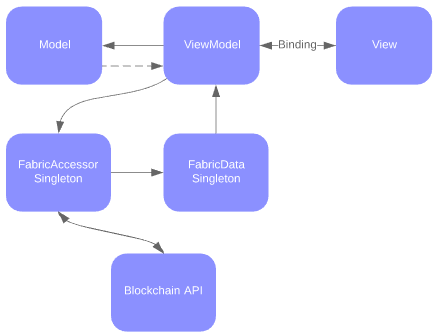
\includegraphics[width=(0.7\textwidth),keepaspectratio]{img/vortex_bc.png}
                \caption{Architecture of user module}
                \label{obr 1.2.1}
            \end{center}
        \end{minipage}
    \end{center}
\end{figure}

Data is stored in the \inlinecode{FabricDataSingleton} so if user creates a company a new object is accessible from other ViewModels immediately. This module displays necessary data for the user to interact with the ledger, displays latest transactions and logs.

\begin{figure}[H]
    \begin{center}
        \begin{minipage}{\linewidth}
            \begin{center}
                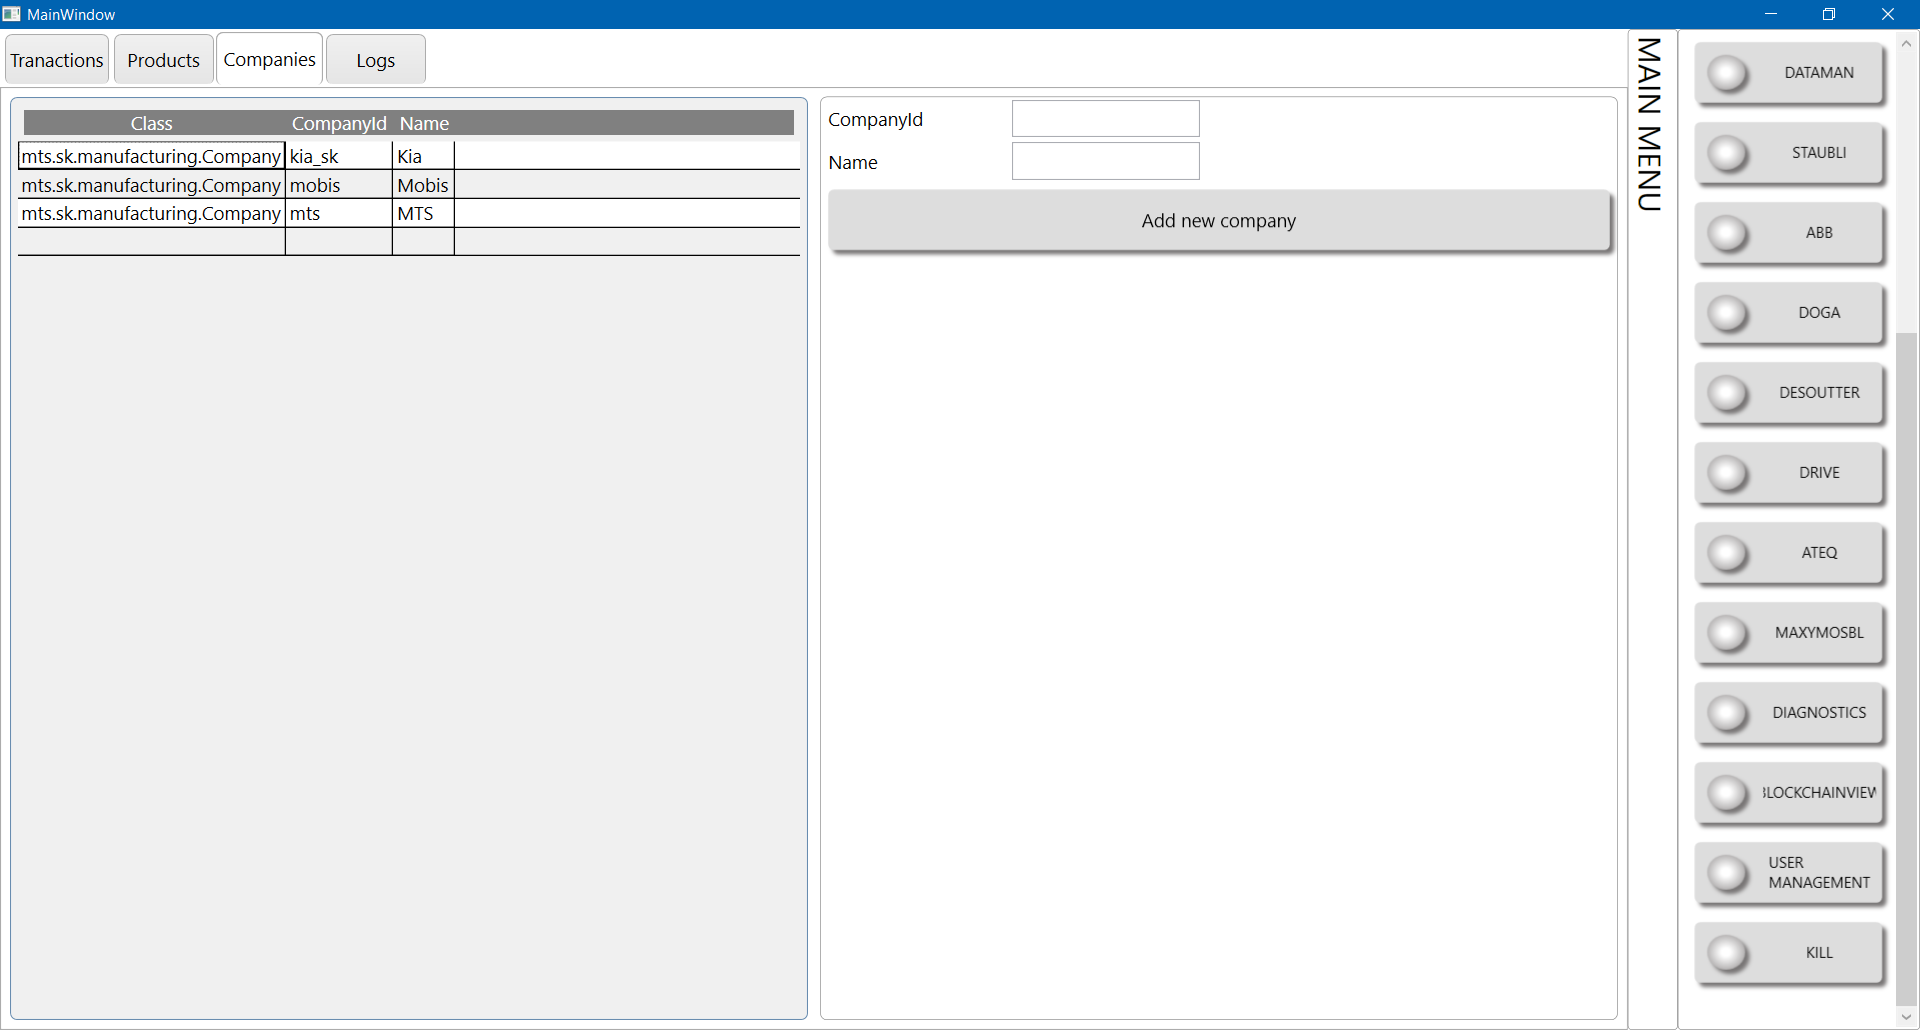
\includegraphics[width=(0.8\textwidth),keepaspectratio]{img/app/vortex_companies.png}
                \caption{Screenshot from application - companies}
                \label{obr 1.2.1}
            \end{center}
        \end{minipage}
    \end{center}
\end{figure}

\begin{figure}[H]
    \begin{center}
        \begin{minipage}{\linewidth}
            \begin{center}
                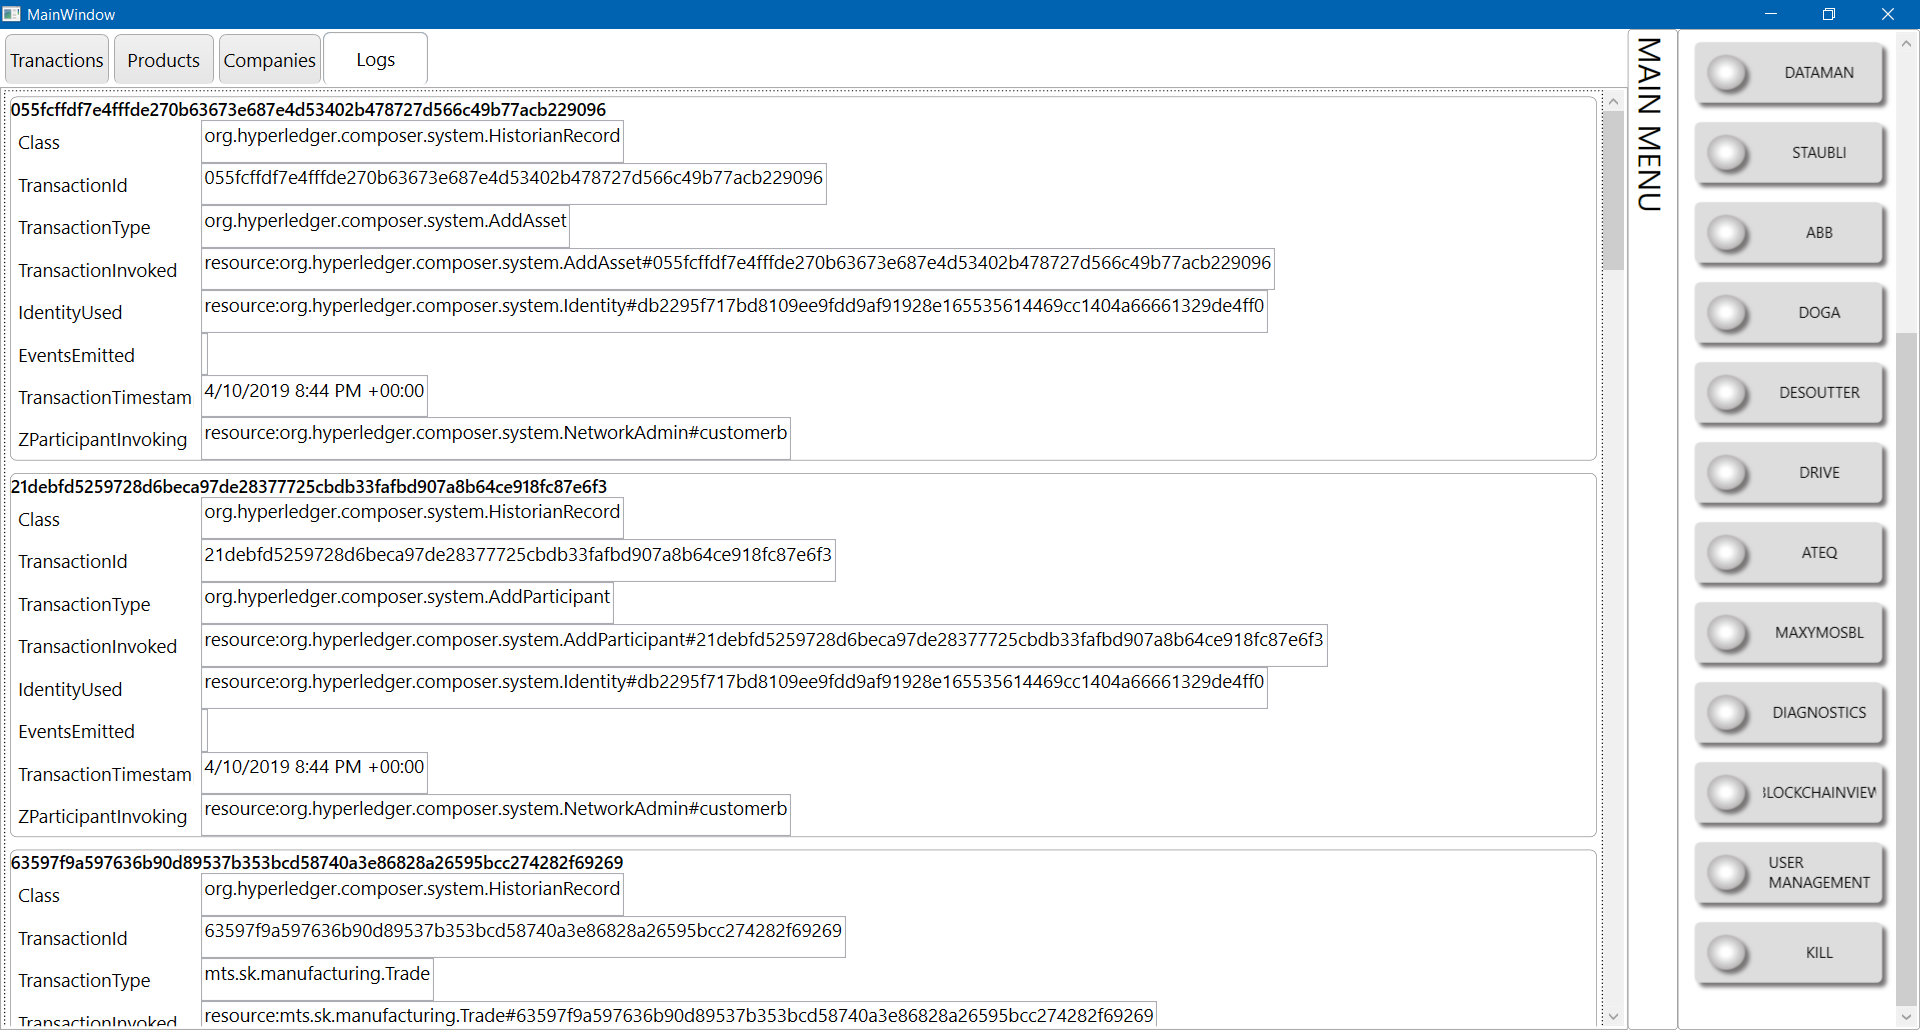
\includegraphics[width=(0.8\textwidth),keepaspectratio]{img/app/vortex_logs.png}
                \caption{Screenshot from application - logs}
                \label{obr 1.2.1}
            \end{center}
        \end{minipage}
    \end{center}
\end{figure}

\begin{figure}[H]
    \begin{center}
        \begin{minipage}{\linewidth}
            \begin{center}
                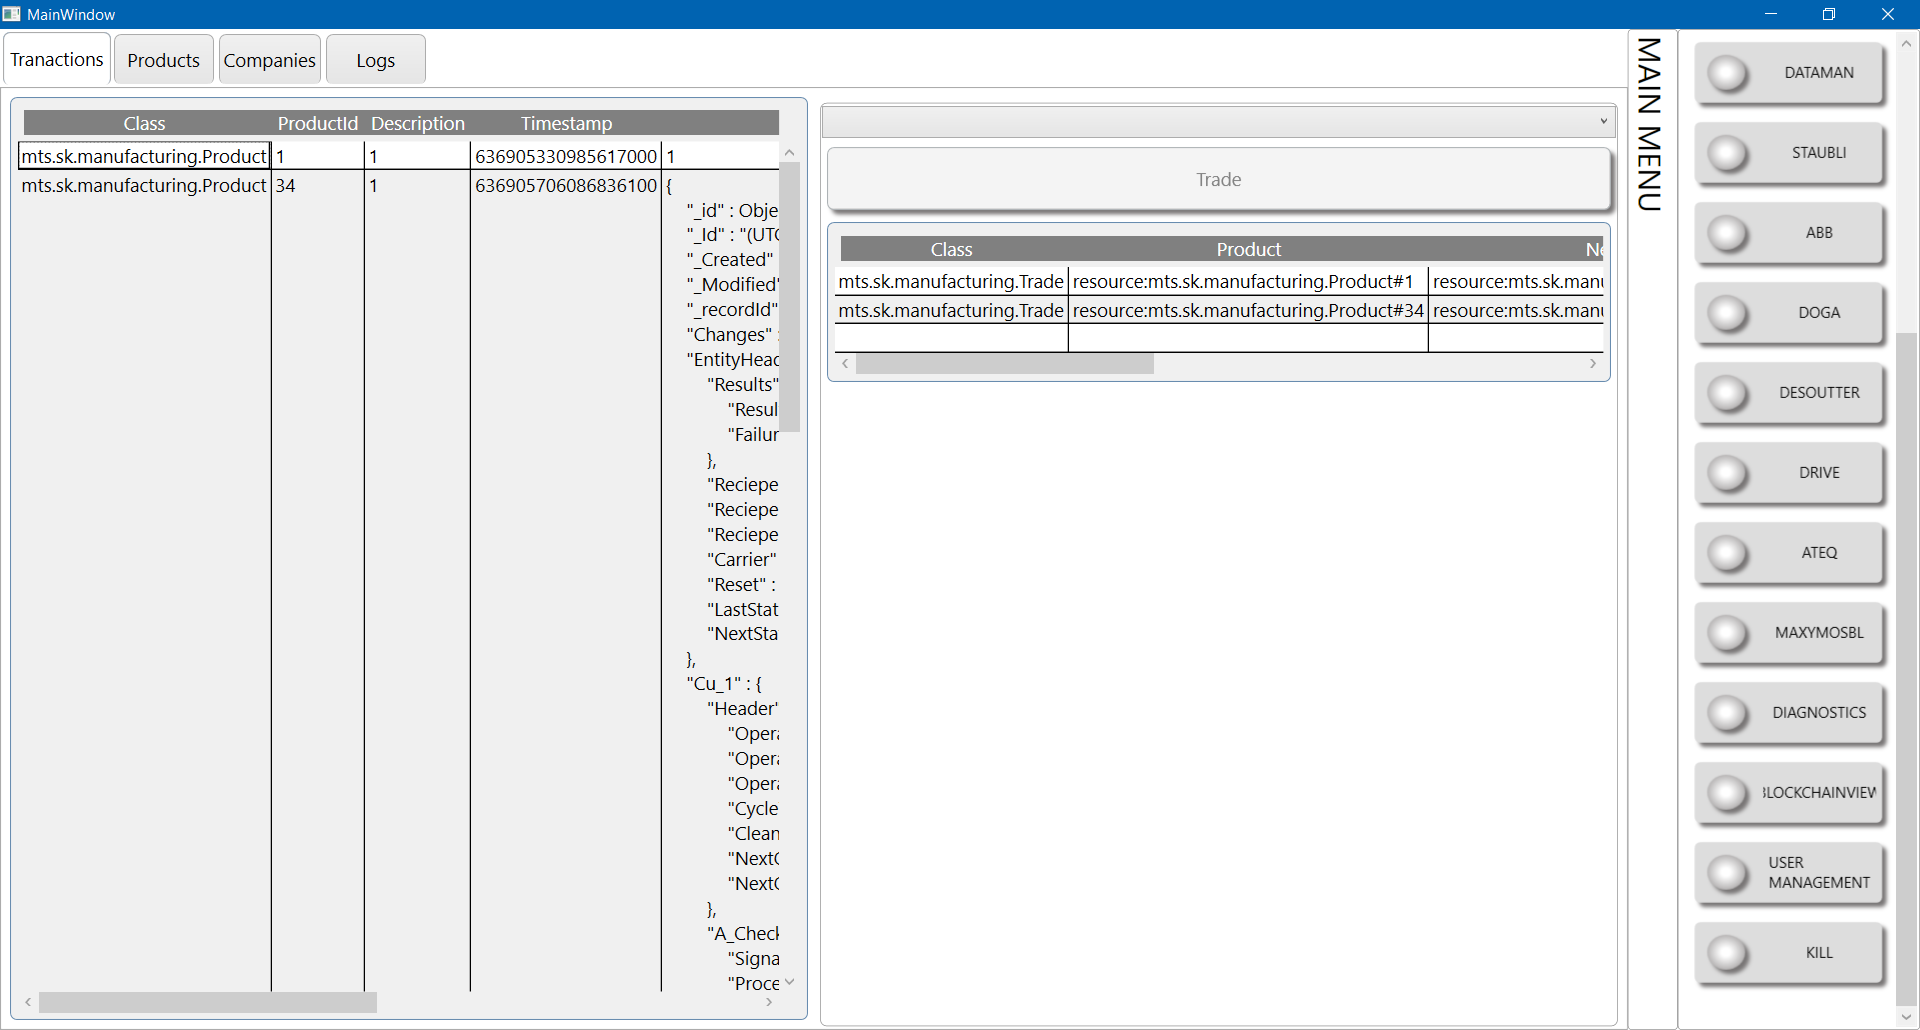
\includegraphics[width=(0.8\textwidth),keepaspectratio]{img/app/vortex_transaction.png}
                \caption{Screenshot from application - transactions}
                \label{obr 1.2.1}
            \end{center}
        \end{minipage}
    \end{center}
\end{figure}


